Nous avons effectué plusieurs séries de tests selon les critères de l'énoncé, c'est à dire :
\begin{itemize}
 \item Effectuer des tests exhaustifs jusqu'à atteindre une résolution totale supérieure à 3 minutes
 \item Effectuer ensuite des tests aléatoires jusqu'à une résolution totale supérieure à 3 minutes (quelque soit le nombre de test)
\end{itemize}
Nous avons, en revanche, lorsque la résolution nous obtenait un résultat légèrement supérieur à 3 minutes, ajouté une ligne supplémentaire dans le tableau.
\subsection{Algorithme 1}
\begin{table}[p]
{%
\begin{center}
\begin{tabular}{||p{1cm}||p{2.5cm}|p{2.5cm}|p{2.5cm}|p{2.5cm}|p{2.5cm}||}
\hline\hline
\multicolumn{6}{||c||}{Algorithme $A_1$ - Temps d'exécution}\\\hline\hline
$n$ & Nombre de & Analyse& \multicolumn{3}{c||}{Temps d'exécution}\\
& tests effectués & exhaustive ?  &Au mieux&en moyenne&au pire\\\hline\hline


1 & 10 & OUI& 0,000 ms & 0,000 ms & 0,000 ms\\\hline
2 & 136 & OUI & 0,000 ms & 0,000 ms & 0,000 ms\\\hline
4 & 32896 & OUI & 0,000 ms & 0,000 ms & 0,000 ms\\\hline
8 & 975800000 & NON & 0,000 ms & 0,000 ms & 0,000 ms\\\hline
10 & 614000000 & NON & 0,000 ms & 0,000 ms & 0,000 ms\\\hline
20 & 171270000 & NON & 0,000 ms & 0,001 ms & 0,002 ms\\\hline
40 & 40520000 & NON & 0,004 ms & 0,004 ms & 0,005 ms\\\hline
80 & 9656000 & NON & 0,012 ms & 0,019 ms & 0,024 ms\\\hline
100 & 6047000 & NON & 0,024 ms & 0,030 ms & 0,036 ms\\\hline
200 & 1438500 & NON & 0,080 ms & 0,125 ms & 0,170 ms\\\hline
400 & 351200 & NON & 0,440 ms & 0,513 ms & 0,570 ms\\\hline
800 & 86690 & NON & 1,600 ms & 2,076 ms & 2,500 ms\\\hline
1000 & 55300 & NON & 2,800 ms & 3,255 ms & 3,700 ms\\\hline
2000 & 10583 & NON & 0,000 ms & 17,009 ms & 29,000 ms\\\hline
4000 & 2800 & NON & 36,000 ms & 64,287 ms & 92,000 ms\\\hline
8000 & 721 & NON & 161,000 ms & 249,953 ms & 293,000 ms\\\hline
10000 & 464 & NON & 325,000 ms & 388,560 ms & 445,000 ms\\\hline
20000 & 117 & NON & 1448,000 ms & 1543,350 ms & 1653,000 ms\\\hline
40000 & DM & NON & DM & DM & DM\\\hline\hline
\end{tabular}
\caption{Résultats expérimentaux de l'algorithme 1}
\label{tab1}
\end{center}
}%
\end{table}
Les mesures présentée dans le tableau \ref{tab1} ont été effectuées avec le système de facteur présenté en partie \ref{facteur}.
Les faibles mesures (seulement une ligne au dessus de la seconde) nous impose une présentation des résultats en millisecondes.
On remarque que l'algorithme effectue un dépassement mémoire à partir de $n=40 000$. Si l'on considère un caractère encodé en 8 bits, la matrice générée est alors de $40000*40000$ octets, soit environ 6 Gibioctets de mémoire.
On s'apercoit néanmoins que cet algorithme est très rapide, comme en témoigne le graphique \ref{graphalgo1}
\begin{figure}[p]
  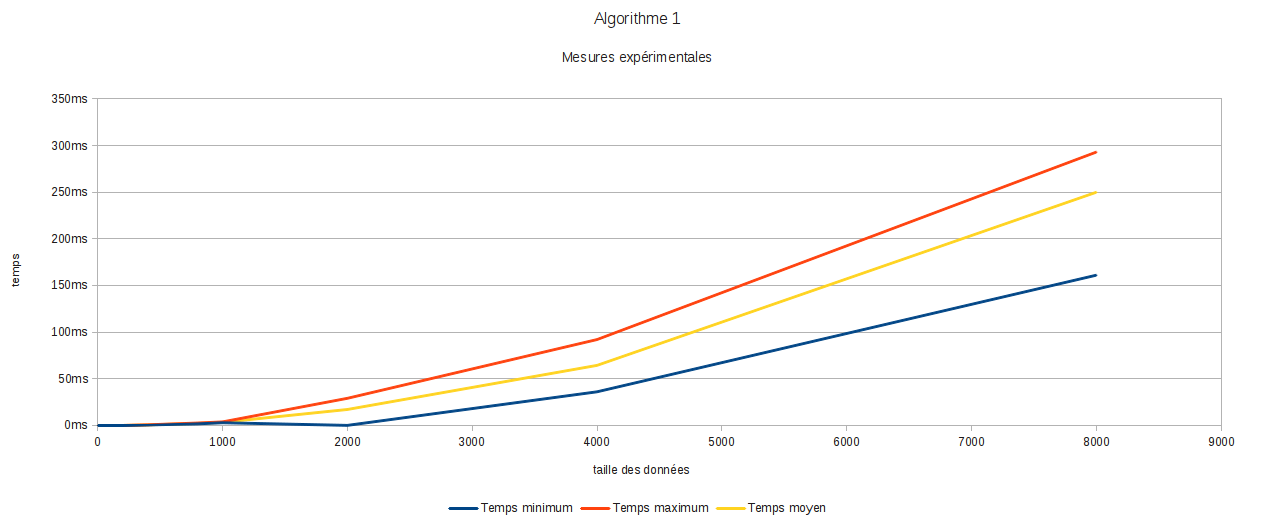
\includegraphics[width=\textwidth]{expe_algo1}
  \caption{Représentation graphique des résultats expérimentaux de l'algorithme 1}
    \label{graphalgo1}
\end{figure}

\subsection{Algorithme 2}
\begin{table}[p]
{%
\begin{center}
\begin{tabular}{||p{1cm}||p{2.5cm}|p{2.5cm}|p{2.5cm}|p{2.5cm}|p{2.5cm}||}
\hline\hline
\multicolumn{6}{||c||}{Algorithme $A_2$ - Temps d'exécution}\\\hline\hline
$n$ & Nombre de & Analyse& \multicolumn{3}{c||}{Temps d'exécution}\\
& tests effectués & exhaustive ?  &Au mieux&en moyenne&au pire\\\hline\hline

1 & 10 & OUI & 0,000 ms & 0,000 ms & 0,000 ms\\
2 & 136 & OUI & 0,000 ms & 0,000 ms & 0,000 ms\\
4 & 32896 & OUI & 0,000 ms & 0,000 ms & 0,000 ms\\
8 &  87115000 & NON & 0,001 ms & 0,002 ms & 0,004 ms\\
10 & 46420000 & NON & 0,002 ms & 0,004 ms & 0,005 ms\\
20 & 6246000 & NON & 0,016 ms & 0,029 ms & 0,040 ms\\
40 & 778800 & NON & 0,160 ms & 0,231 ms & 0,340 ms\\
80 & 93900 & NON & 1,760 ms & 1,917 ms & 2,080 ms\\
100 & 48450 & NON & 3,520 ms & 3,719 ms & 3,920 ms\\
200 & 5907 & NON & 20,000 ms & 30,474 ms & 33,000 ms\\
400 & 725 & NON & 240,000 ms & 248,346 ms & 257,000 ms\\
800 & 90 & NON & 1993,000 ms & 2014,560 ms & 2036,000 ms\\
1000 & 46 & NON & 3905,000 ms & 3931,000 ms & 3965,000 ms\\
2000 & 6 & NON & 31273,000 ms & 31313,800 ms & 31406,000 ms\\
4000 & 1 & NON & 252191,000 ms & 252191,000 ms & 252191,000 ms\\\hline\hline
\end{tabular}

\caption{Résultats expérimentaux de l'algorithme 2}

\label{tab2}
\end{center}
}%
\end{table}

La forme de l'algorithme 2 nous laisse à penser que les coûts aux pire et au mieux sont identiques. En effet, $A_2$ est constitué de trois boucles indépendantes de la forme des données, seule la taille compte. En parcourant et comparant la liste de toutes les sous-chaînes possibles, le temps d'exécution sera toujours constant, quelque soit le résultat retourné.
Les courbes confondues dans la figure \ref{graphalgo2} le prouvent. L'algorithme est toutefois plus lent que le premier, car une seule comparaison de deux chaînes de 4000 caractère prend environ 4 minutes.


\begin{figure}[p]
  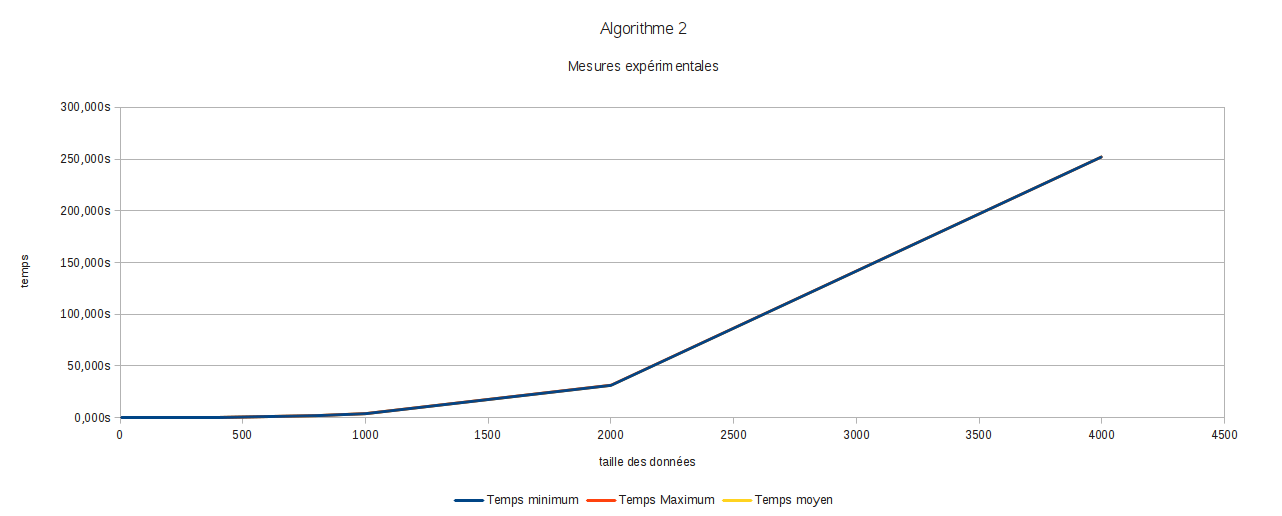
\includegraphics[width=\textwidth]{expe_algo2}
  \caption{Représentation graphique des résultats expérimentaux de l'algorithme 2}
    \label{graphalgo2}
\end{figure}

\subsection{Algorithme 3}
\begin{table}[p]
{%
\begin{center}
\begin{tabular}{||p{1cm}||p{2.5cm}|p{2.5cm}|p{2.5cm}|p{2.5cm}|p{2.5cm}||}
\hline\hline
\multicolumn{6}{||c||}{Algorithme $A_2$ - Temps d'exécution}\\\hline\hline
$n$ & Nombre de & Analyse& \multicolumn{3}{c||}{Temps d'exécution}\\
& tests effectués & exhaustive ?  &Au mieux&en moyenne&au pire\\\hline\hline

1 & 10 & NON & 0,000s & 0,000s & 0,000s\\
2 & 136 & NON & 0,000s & 0,000s & 0,000s\\
4 & 12131 & NON & 0,000s & 0,000s & 0,000s\\
8 & 43050000 & OUI & 0,000s & 0,000s & 0,000s\\
10 & 25040000 & OUI & 0,000s & 0,000s & 0,000s\\
20 & 3987800 & OUI & 0,000s & 0,000s & 0,000s\\
40 & 579700 & OUI & 0,000s & 0,000s & 0,000s\\
80 & 79300 & OUI & 0,002s & 0,002s & 0,002s\\
100 & 41190 & OUI & 0,003s & 0,004s & 0,005s\\
200 & 5276 & OUI & 0,028s & 0,034s & 0,037s\\
400 & 665 & OUI & 0,260s & 0,271s & 0,280s\\
800 & 84 & OUI & 2,136s & 2,163s & 2,200s\\
1000 & 43 & OUI & 4,200s & 4,265s & 4,329s\\
2000 & 6 & OUI & 33,727s & 33,936s & 34,134s\\
4000 & NRP & OUI & NRP & NRP & NRP\\\hline\hline
\end{tabular}

\caption{Résultats expérimentaux de l'algorithme 3}

\label{tab3}
\end{center}
}%
\end{table}
Tout comme pour l'algorithme $A_2$, les courbes de temps au mieux/au pire de l'algorithme $A_3$ sont confondues. 
Il serait pertinent de vérifier que le temps d'exécution ne dépend pas de la forme des données, mais le manque de compréhension de cet algorithme nous empêche de confirmer cette hypothèse.
\begin{figure}[p]
  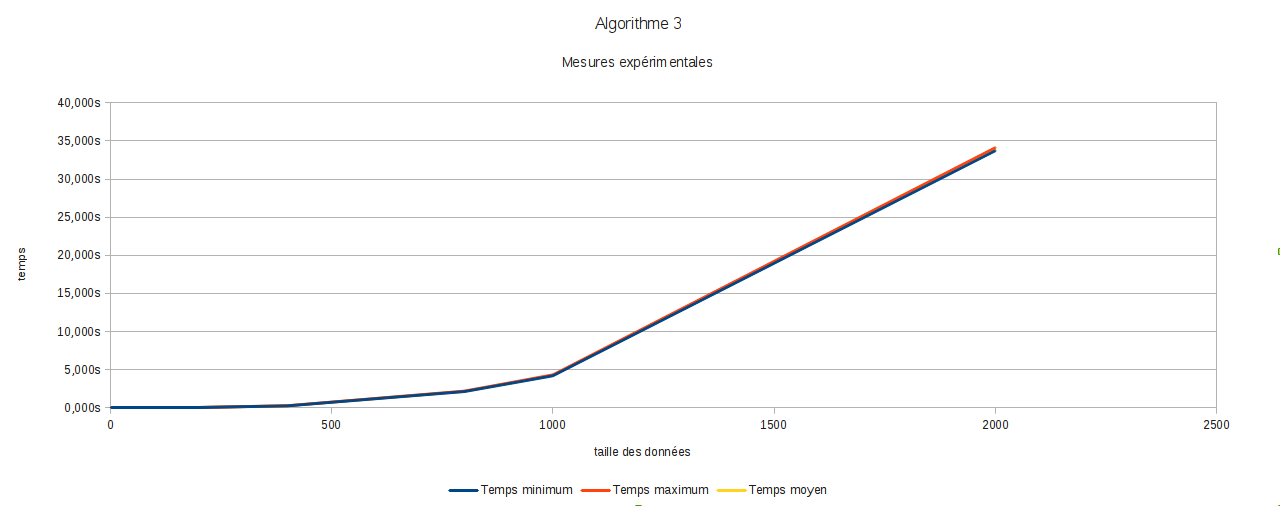
\includegraphics[width=\textwidth]{expe_algo3}
  \caption{Représentation graphique des résultats expérimentaux de l'algorithme 3}
    \label{graphalgo3}
\end{figure}